\documentclass[../main.tex]{subfiles}
\begin{document}

There exist several applications where the complexity and volume of the task requires crowdsourcing to a large set of human labelers.
Inferring the true label of an item from the labels assigned by several labelers is facilitated by this crowdsourced annotation model\cite{passonneau2014benefits}.
The model takes into consideration an unknown prevalence of label categories, an unknown per-item category, and an unknown confusion matrix per-labeler.

The model is shown in plate notation in figure\ref{fig:fig4} \newline
\begin{figure}[h]
  \centering
  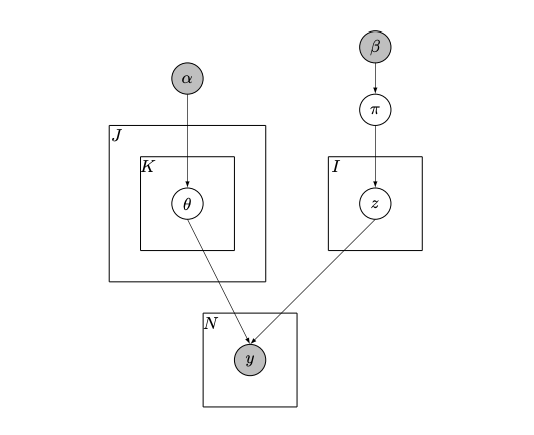
\includegraphics[width=100mm]{plate_notation_crowdsourced_annotation.png}
  \caption{Plate notation of crowdsourced annotation model\cite{passonneau2014benefits}}
  \label{fig:fig4}
\end{figure}

Let $K$ be the number of possible labels or categories for an item, $I$ the number of items to annotate, $J$ the number of labelers, and $N$ the total number of labels provided by labelers.Each item is labeled by at least one labeler.\newline
The parameters of the model are as follows:
\begin{itemize}
\item $z_i \in 1:K$ for the true category of item $i$,
\item $\pi_k \in [0, 1]$ for the probability that an item is of
category $k$.
\item $\theta_{j,k,k'} \in [0, 1]$ for the probabilty that annotator $j$ assigns the label $k'$ to an item whose true category is $k$;
Subject to $\sum_{k'=1}^{K}theta_{j,k,k'} = 1$
\end{itemize}
The model first selects the true category $z_i$ for item $i$ according to the prevalence $\pi$ of categories where,
$$
\pi \sim Dirichlet(\beta);
$$
and,
$$
z_i \sim Categorical(\pi)
$$
Each item $i$ is labelled by $|J_i|$ labelers, where
$$
|J_i| \sim Poisson(\lambda_{labeler})
$$
These labelers are choosen at random from all the labelers
$$
J_i \sim Categorical(J, |J_i|)
$$
For each labeler $j$ the confusion matrix $\theta_{j,k}$,(k) is sampled from dirichlet prior $\alpha_k$, where
$$
\alpha_{k,k} = E_{correctness}, \quad \alpha_{k,k'} = (1- E_{correctness})/(K-1)
$$
Here, $E_{correctness}$ denotes the expected proportion of times the labeler correctly identifies the true label.
$\theta_{j,k}$ for each labeler is sampled as follows:
$$
\theta_{j,k} \sim Dirichlet(\alpha_k)
$$
The label $y_n$ for item $i$ is sampled from the labeler $j$'s confusion matrix $\theta_{j,z[i]}$
$$
y_n \sim Categorical(\theta_{J_{i[n]}, z_i})
$$

\subsection{Data Generation}
For the experiment, we simulate a model with $|J| = 100$ labelers, $|I| = 5000$ items, and $|K| = 3$ categories. The hyperprior configuration is listed in table \ref{tab:table_CSA}.
The labels of half of the items are passed to the PPL implementations for training and the other half is used to compute the posterior predictive of the obtained samples.
\begin{table}[h]
 \caption{Hyperpriors for Crowdsourced Annotation Model}
  \centering
  \begin{tabular}{lll}              \\
    \cmidrule(r){1-3}
    Hyperprior             & Value            & Notes  \\
    \midrule
    $\lambda_{labeler}$    & 2.5              & Poisson prior for number of labelers assigned to each item    \\
    $\beta$                & [$\frac{1}{K}$]  & Dirichlet prior for $\pi$ \\
    $E_{correctness}$        & 0.5              & Expected accuracy of a labeler    \\
    \bottomrule
  \end{tabular}
  \label{tab:table_CSA}
\end{table}
\subsection{PPL Implementations}
The model was implemented in Stan and Jags PPLs, with the help of PyStan\cite{PyStan} and PyJAGS\cite{PyJAGS} libraries for interface.
The compilation and inference times were recorded.
The model requires the support for discrete latent vairables, which JAGS has, but Stan does not.
This means that the Stan implementation requires an additional marginaliztion step w.r.t $z[i]$, the true label of each item.

\begin{figure}[h]
  \centering
  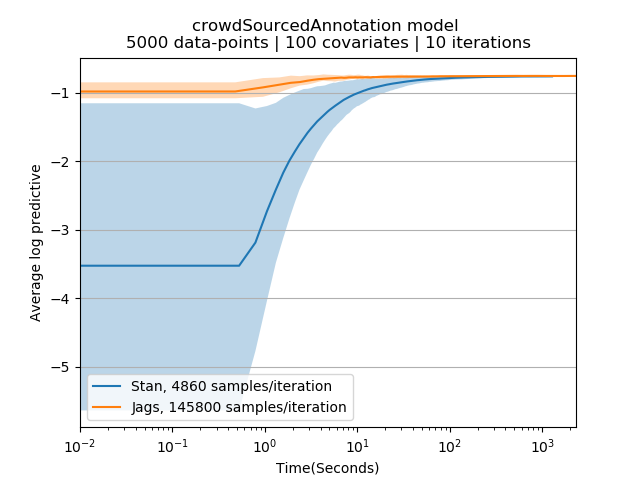
\includegraphics[width=150mm]{../figures/analysis_crowdsourced_annotation.png}
  \caption{Posterior convergence behaviour of Jags and Stan for Crowdsourced Annotation Model}
  \label{fig:fig2}
\end{figure}

\subsection{Results}
Figure \ref{fig:fig2} shows the comparative performance.
From the figure, we can make the following observations:
\begin{itemize}
\item Both implementations converge to the same posterior predictive log-likelihood given enough time.
\item Jags is both faster to converge as well has a much lower time per sample.
\item Jags' inference starts sampling from relatively high log-likelihood space  and hence converges much quicker than STAN's
\end{itemize}

\bibliographystyle{unsrt}
\bibliography{../references}

\end{document}
